% %%%%%%%%%%%%%%%%%%%%%%%%%%%%%%%%%%%%%%%%%%%%%%%%%%%%%%%%%%%%%%%%%%%%%
% %% Microarchitecture %%
% Microarchitecture
% %%%%%%%%%%%%%%%%%%%%%%%%%%%%%%%%%%%%%%%%%%%%%%%%%%%%%%%%%%%%%%%%%%%%%



%% add RAM, nop, RTL, CAM



\section{Microarchitecture}
\label{sec:arch:microarch}

% In light of the above analysis, this section describes the architecture of a \gls{redC} capable of supporting multiple regions with distinct characteristics.
% We introduce OBaMMA, an \textit{\underline{O}uter-Product} \underline{Ba}nded \underline{M}atrix \underline{M}emory \underline{A}ccelerator.
\acrlong{spdc} features two primary capabilities.
First, as a \gls{redC}, it supports \textit{reduction} instructions, enabling the accumulation of data near-memory.
Second, it implements a region-based cache where regions have different data-granularity, levels of associativity and overall behavior.

% The OBaMMA cache has three regions:
% \begin{itemize}
%     \item The \acrshort{grc} (\textit{Generic Region Cache}) functions as a generic cache region.
%     It is useful for processing sequential memory accesses that occur during the computation of sparse kernels.
%     For example, in the \algo{OP} SpMV kernel, the \acrshort{grc} manages the sequential reads of matrix $A$ and vector $b$.
%     %
%     \item The \acrshort{drc} (\textit{Dense Region Cache}) operates as a line-wise set-associative \gls{redC}.
%     It exclusively processes \textit{reduction} instructions, in a write-back manner.
%     Data to be accumulated is held only in the cache.
%     Memory transactions, to synchronize main memory, are issued only on data \gls{eviction}.
%     This region is beneficial for matrix areas which exhibit high locality despite the apparent randomness of accesses, such as within the matrix band.
%     %
%     \item The \acrshort{srt} (\textit{Sparse Region Table}) functions as an element-wise fully-associative \gls{redC}.
%     Like the \acrshort{drc}, it processes \textit{reduction} instructions in a write-back manner but employs atomic element-wise memory transactions instead of the conventional line-wise read and write transactions.
%     This region is advantageous for matrix areas where elements are isolated, having minimal spatial locality, such as outside the band of a matrix.
% \end{itemize}

% This approach is similar to~\cite{Isaac2024_SpDCache} which already suggested that splitting a cache can reduce memory traffic, however, the analysis was empirical, based on a high-level Python model and the sizing of the regions was not addressed.
% Our work extends this by providing an analytical study that strengthens the concept and offers insights into region dimensioning.
% Additionally, OBaMMA includes a fully functional RTL implementation, enabling accurate performance and area evaluation, as presented in Section~\ref{sec:evaluation}.

\subsection{HPDcache: The RTL base generic cache}

\acrlong{spdc} is implemented into an L1 data cache for a CVA6 RISC-V core, building upon an existing open-source high-performance set-associative data cache known as HPDcache~\cite{Fuguet2023_HPDcache}.
In contrast to traditional data caches, HPDcache introduces new features, including buffering techniques for memory writes, set-associative storage to manage read \gls{miss} requests, and dynamic configurability of each cache-line to operate in either write-back or write-through modes.
It is designed for high performance, utilizing a three-stage pipeline to handle multiple instructions while minimizing stall potential through out-of-order cache execution.

An overview of \acrlong{spdc}'s microarchitecture is shown in Figure~\ref{fig:arch:microarch}, where \textit{black} and \textit{blue} components are originally from HPDcache.
The first stage (\textit{st0}) decodes instructions and issues reads to the cache directory and data RAMs (\textit{Dir} and \textit{Data}).
These reads require one cycle to respond.
In the second stage (\textit{st1}), the response indicates whether a \gls{hit} or \gls{miss} occurred and if an \gls{eviction} is necessary.
The instruction proceeds to the final stage (\textit{st2}) only if a \gls{miss} or \gls{eviction} must be processed.
At \textit{st0}, the instruction is not yet consumed.
Depending on the response and the availability of cache resources at \textit{st1}, a \textit{nop} (\textit{no operation}) may be inserted in the pipeline, and the instruction may be placed in a \textit{replay table}.
The instruction is then replayed with the highest priority once its dependencies are cleared.
If the instruction does not need to be replayed at \textit{st1}, it is consumed and processed.
This pipeline serves as the foundation for implementing \acrlong{spdc}'s \gls{reduction} operations.
% add infos on blocks such as UC, CMO..

HPDcache provides extensive static and dynamic configurability, making it a flexible foundation for further extensions.
To implement \acrlong{spdc} as well as a \gls{redC} baseline, we modified HPDcache to be highly configurable so that a single RTL implementation can produce multiple designs.
The RTL can be instantiated as a generic cache (the first baseline, \acrshort{gc}), as a \gls{redC} (the second baseline, \acrshort{redc}), or as \acrshort{spdc}, the solution presented in the previous chapters.

\subsection{RTL Implementation of SpDCache}

We configure the original HPDcache as a 4-way set-associative cache with 128 \glspl{set} and 64-byte cache-lines, resulting in a total cache size of 32~KiB.
We extend the three-stage pipeline to handle the new \gls{red} instruction.
Figure~\ref{fig:arch:microarch} provides an overview of \acrlong{spdc}'s microarchitecture, highlighting new blocks in \textit{red}, modified blocks in \textit{blue}, and untouched components in \textit{black}.
The overall architecture aligns with the design presented in Chapter~\ref{cha:spdc}, adapted here for hardware implementation.
Let us briefly describe the operation of the \acrshort{drc} under three scenarios: \glspl{hit}, \glspl{miss} with available cache-lines, and \glspl{miss} requiring \gls{eviction}.

\begin{figure}[htbp]
    \centering
    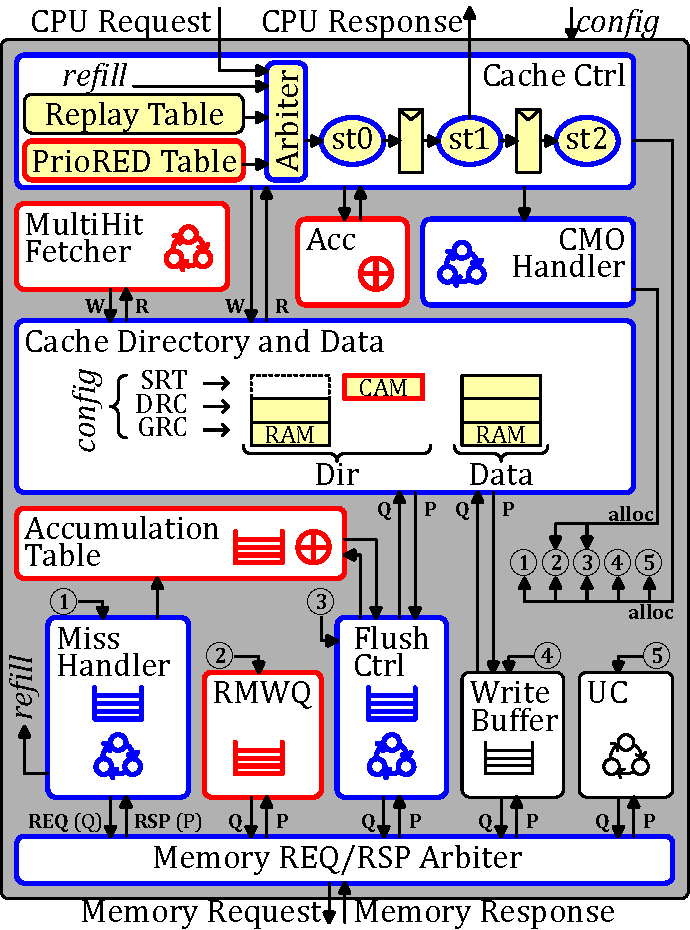
\includegraphics[width=0.7\linewidth]{Chapter_MicroArch/Figures/PDF/SpDC_MicroArchi.pdf}
    \caption{\acrlong{spdc} Microarchitecture, based on HPDcache \note{RMWQ}}
    \label{fig:arch:microarch}
\end{figure}

\textbf{In the case of a \gls{hit}}, the value of the \gls{red} instruction is accumulated with its corresponding value in the cache.
At \textit{st1}, the cache value, read in \textit{st0} from \textit{Data}, is accumulated with the \gls{red} value using a dedicated accumulator (\textit{Acc}).
The result is written back to \textit{Data} at \textit{st2}.

\textbf{In the case of a \gls{miss}}, if there is an available cache-line, the value of the \gls{red} instruction is simply stored in this free entry of the cache.
A free cache-line is selected at \textit{st1}, and at \textit{st2}, the \gls{red} value is written to \textit{Data} along with zeros to reset the selected cache-line.
A write to \textit{Dir} is also performed to change the state of the cache-line from free to valid.

\textbf{If a \gls{miss} occurs but no cache-line is free}, an \gls{eviction} must be processed before handling the \gls{red} instruction.
The \gls{red} instruction is placed in the \textit{PrioRED table} to be replayed with higher priority than the \textit{replay table}.
Meanwhile, at \textit{st2}, the \textit{miss handler}, \textit{flush controller}, and \textit{accumulation table} are allocated to process the \gls{eviction}.
The \gls{eviction} is a ``fire-and-forget'' operation, meaning the \gls{red} instruction only needs to wait for the entry in \textit{Data} to be freed, not for the entire \gls{eviction} to finish.
The \gls{eviction} process begins by fetching and resetting the chosen 64~B cache-line from \textit{Data}, which is done in one cycle by the \textit{flush controller}.
Simultaneously, the \textit{miss handler} issues a read to the main memory, which in our performance simulations, we assume will take 64 cycles to respond. \note{FIX}
The \textit{accumulation table} waits and temporarily stores both the old cache-line from the \textit{flush controller} and the 64~B response data from the \textit{miss handler}.
It then accumulates the cache-line with the data, word by word, and sends the 64~B results back to the main memory using the existing write interface.

With the changes described above, we have transformed \mbox{HPDcache} into a \gls{redC}.
To achieve multiple cache regions, we virtually separate the cache RAMs.
To maintain HPDcache's set-associative operation, we divide the cache memory along its \glspl{set}.
Thus, each region of the cache has the same structure as the overall cache but is smaller in size: each \gls{set} contains a fixed number (the number of ways) of 64-byte cache-lines, as depicted in Figure~\ref{fig:arch:set_redirection}.
Each region can map any possible address.
To ensure that every address matches a unique \gls{set} within each region, we allocate a power-of-two number of consecutive \glspl{set} to a region.
Considering the total number of \glspl{set} $S_T$ and our region $R$ mapping on $S_R < S_T$ of them, starting at the \gls{set} $s_\mathit{offset}$, if an address matches one of the \glspl{set} of this region, no action is required.
However, if the address matches a \gls{set} $s_\mathit{addr}$ outside the region, we need to map it to a unique \gls{set} in the region such that $s_\mathit{region} = (s_\mathit{addr} \% S_R) + s_\mathit{offset}$, as illustrated in Figure~\ref{fig:arch:set_redirection}.
The three regions \acrshort{grc}, \acrshort{drc}, and \acrshort{srt} are each defined by their number of \glspl{set} $S_R$ and their first \gls{set}, $s_\mathit{offset}$.
\acrlong{spdc} can thus be reconfigured to operate as a generic cache, a traditional \gls{redC} or a region-based \gls{redC} based on the needs of the application (\textit{config} in Figure~\ref{fig:arch:microarch}).

\begin{figure}[htbp]
    \centering
    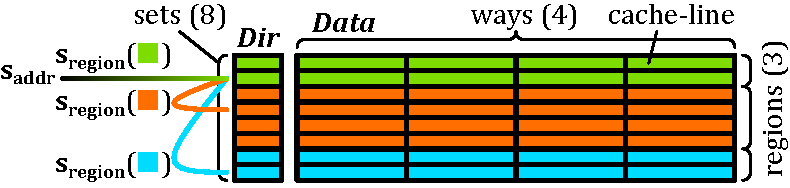
\includegraphics[width=\linewidth]{Chapter_MicroArch/Figures/PDF/Sets_redirection.pdf}
    \caption{Set Redirection Depending on the Region}
    \label{fig:arch:set_redirection}
\end{figure}

The \acrshort{srt} region requires additional adjustments to function as an element-wise fully-associative cache.
This region operates as if all the \glspl{set} were combined into a single \gls{set}, containing numerous elements.
Each element requires its own directory entry.
Therefore, we replace the \textit{Dir} RAMs of this region with a \textit{CAM} (\textit{Content-Addressable Memory}) containing the addresses of each valid element in the \acrshort{srt} region.
With the \textit{CAM}, we can check for a \gls{hit} across the entire region and retrieve the matching value stored in the \textit{Data} RAMs.
We also added a queue (\textit{RED AMO Queue}) \note{FIX} to manage the element-wise \gls{rmw} memory transactions.

To avoid address duplication between regions, the \textit{MultiHit fetcher} in Figure~\ref{fig:arch:microarch} manages coherency between the \acrshort{drc} and \acrshort{srt}, following the description in Chapter~\ref{cha:spdc}.
Since software selects the region, this can be necessary.
The \textit{MultiHit fetcher} performs two tasks.
First, given an address, it probes the \textit{CAM} for entries whose cache-line address matches.
If one or more matches are found, it records their positions locally and notifies the \textit{cache controller}.
Second, when activated, the \textit{MultiHit fetcher} gathers the corresponding elements from the \textit{Data} RAMs of the \acrshort{srt} and assembles them into a single 64~B line that will be written into the \acrshort{drc}.

%%%
We have added several custom instructions to the CVA6 RISC-V core~\cite{Waterman2016_RISCV_ISA}.
The primary addition is the \textit{reduction} instruction (\gls{red}), which takes an address and a value as arguments and expects no response.
This instruction is accompanied by a region instruction (\textit{REG}) that specifies in which region subsequent \textit{reductions} should be processed.
We have also added an instruction to flush the \textit{reduction} regions (\acrshort{drc} and \acrshort{srt}) of the cache, which is necessary at the end of the algorithm.
It is performed in the cache by the \textit{CMO handler}.
Finally, we have included an instruction to enable and disable the \textit{reduction} mode of \acrlong{spdc}.

\begin{figure}[htbp]
    \centering
    \begin{subfigure}{0.49\linewidth}
        \centering
        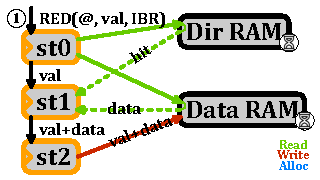
\includegraphics[width=\linewidth]{Chapter_MicroArch/Figures/PDF/SpDC_Pipeline_01.pdf}
        \caption{TODO}
        \label{fig:arch:pipeline_01}
    \end{subfigure}
    \hfill
    \begin{subfigure}{0.49\linewidth}
        \centering
        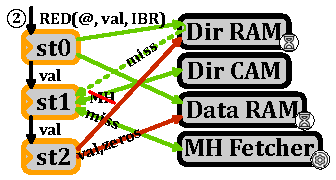
\includegraphics[width=\linewidth]{Chapter_MicroArch/Figures/PDF/SpDC_Pipeline_02.pdf}
        \caption{TODO}
        \label{fig:arch:pipeline_02}
    \end{subfigure}
    %
    \begin{subfigure}{0.49\linewidth}
        \centering
        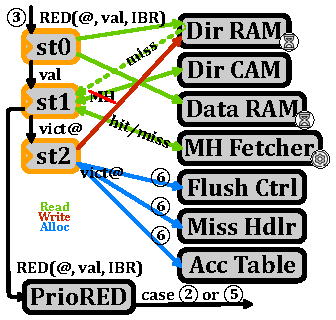
\includegraphics[width=\linewidth]{Chapter_MicroArch/Figures/PDF/SpDC_Pipeline_03.pdf}
        \caption{TODO}
        \label{fig:arch:pipeline_03}
    \end{subfigure}
    \hfill
    \begin{subfigure}{0.49\linewidth}
        \centering
        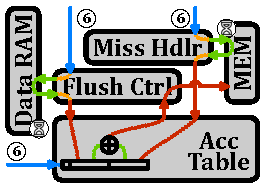
\includegraphics[width=0.8\linewidth]{Chapter_MicroArch/Figures/PDF/SpDC_Pipeline_06.pdf}
        \caption{TODO}
        \label{fig:arch:pipeline_06}
    \end{subfigure}
    %
    \begin{subfigure}{0.49\linewidth}
        \centering
        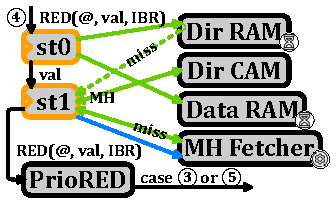
\includegraphics[width=\linewidth]{Chapter_MicroArch/Figures/PDF/SpDC_Pipeline_04.pdf}
        \caption{TODO}
        \label{fig:arch:pipeline_04}
    \end{subfigure}
    \hfill
    \begin{subfigure}{0.49\linewidth}
        \centering
        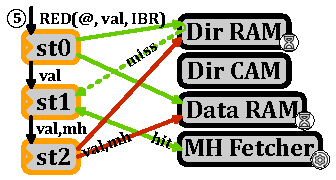
\includegraphics[width=\linewidth]{Chapter_MicroArch/Figures/PDF/SpDC_Pipeline_05.pdf}
        \caption{TODO}
        \label{fig:arch:pipeline_05}
    \end{subfigure}
    \caption{Pipeline Operation IBR}
    \label{fig:arch:pipeline_IBR}
\end{figure}

\begin{figure}[htbp]
    \centering
    \begin{subfigure}{0.49\linewidth} % [position][height][inner pos]{width}
        \centering
        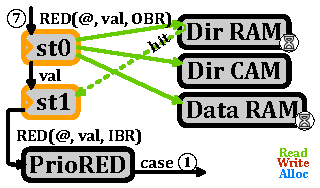
\includegraphics[width=\linewidth]{Chapter_MicroArch/Figures/PDF/SpDC_Pipeline_07.pdf}
        \caption{TODO}
        \label{fig:arch:pipeline_07}
    \end{subfigure}
    \hfill
    \begin{subfigure}{0.49\linewidth}
        \centering
        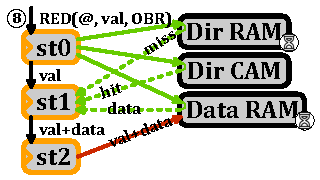
\includegraphics[width=\linewidth]{Chapter_MicroArch/Figures/PDF/SpDC_Pipeline_08.pdf}
        \caption{TODO}
        \label{fig:arch:pipeline_08}
    \end{subfigure}
    %
    \begin{subfigure}{0.49\linewidth}
        \centering
        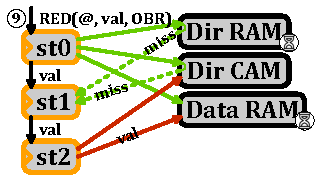
\includegraphics[width=\linewidth]{Chapter_MicroArch/Figures/PDF/SpDC_Pipeline_09.pdf}
        \caption{TODO}
        \label{fig:arch:pipeline_09}
    \end{subfigure}
    \hfill
    \begin{subfigure}{0.49\linewidth}
        \centering
        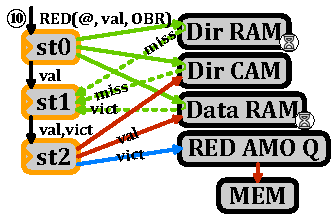
\includegraphics[width=\linewidth]{Chapter_MicroArch/Figures/PDF/SpDC_Pipeline_10.pdf}
        \caption{TODO \note{RMWQ}}
        \label{fig:arch:pipeline_10}
    \end{subfigure}
    \caption{Pipeline Operation OBR}
    \label{fig:arch:pipeline_OBR}
\end{figure}